\section{Webalkalamzás architektúra}
\label{sec:webterv}

Az egész rendszer megtervezése után szüksége volt a felosztott részeknek külön alrendszer tervezésére, amely a \ref{fig:systemArchLittle} ábrán jelenik meg. A tervezés során kideült, hogy négy nagy komponensre lesz szükség: Frontend, Webszerver, Adatbázis és a 3D modell.

Amint az ábrán is látszik a Felhasználók a Frontenden keresztül érik el a teljses alkalmazást. A Frontend fogja bíztosítani a felhasználói felületet, vagyis itt fognak megjelenni az adatok az adatbázisból és a 3D modell is ide fog betöltődni.

A Webszerver segítségével lesznek elérhetőek a Frontend számára az adatbázisban tárolt adatok. Tulajdonképpen a Webszerver biztosít egy kommunikációs csatornát a Frontend és az adatbázis között. A Frontend kéréseket (GET, PUT, POST) küld a webszervernek és a webszerver a kérésnek megfelelő eredményt szolgáltatja vissza.

Az adatbázis fogja tárolni a Frontendről érkező adatokat, valamint vissza is szolgáltatja azokat a megfelelő kérések esetén a Webszerveren keresztül.

A  \ref{sec:rendterv} fejezetben említett 3D modell egy statikus fáljban lesz elhelyezve, amelyet a Frontend ér el és onnan fogja betölteni a modellt egy Frontenden belüli komponensbe. Ezen a komponensen keresztül fog összekapcsolódni a \ref{sec:rendterv} fejezetben említett két alrészleg, maga a webapplikáció és a 3D modell.
\begin{figure}[H]
	\centering
	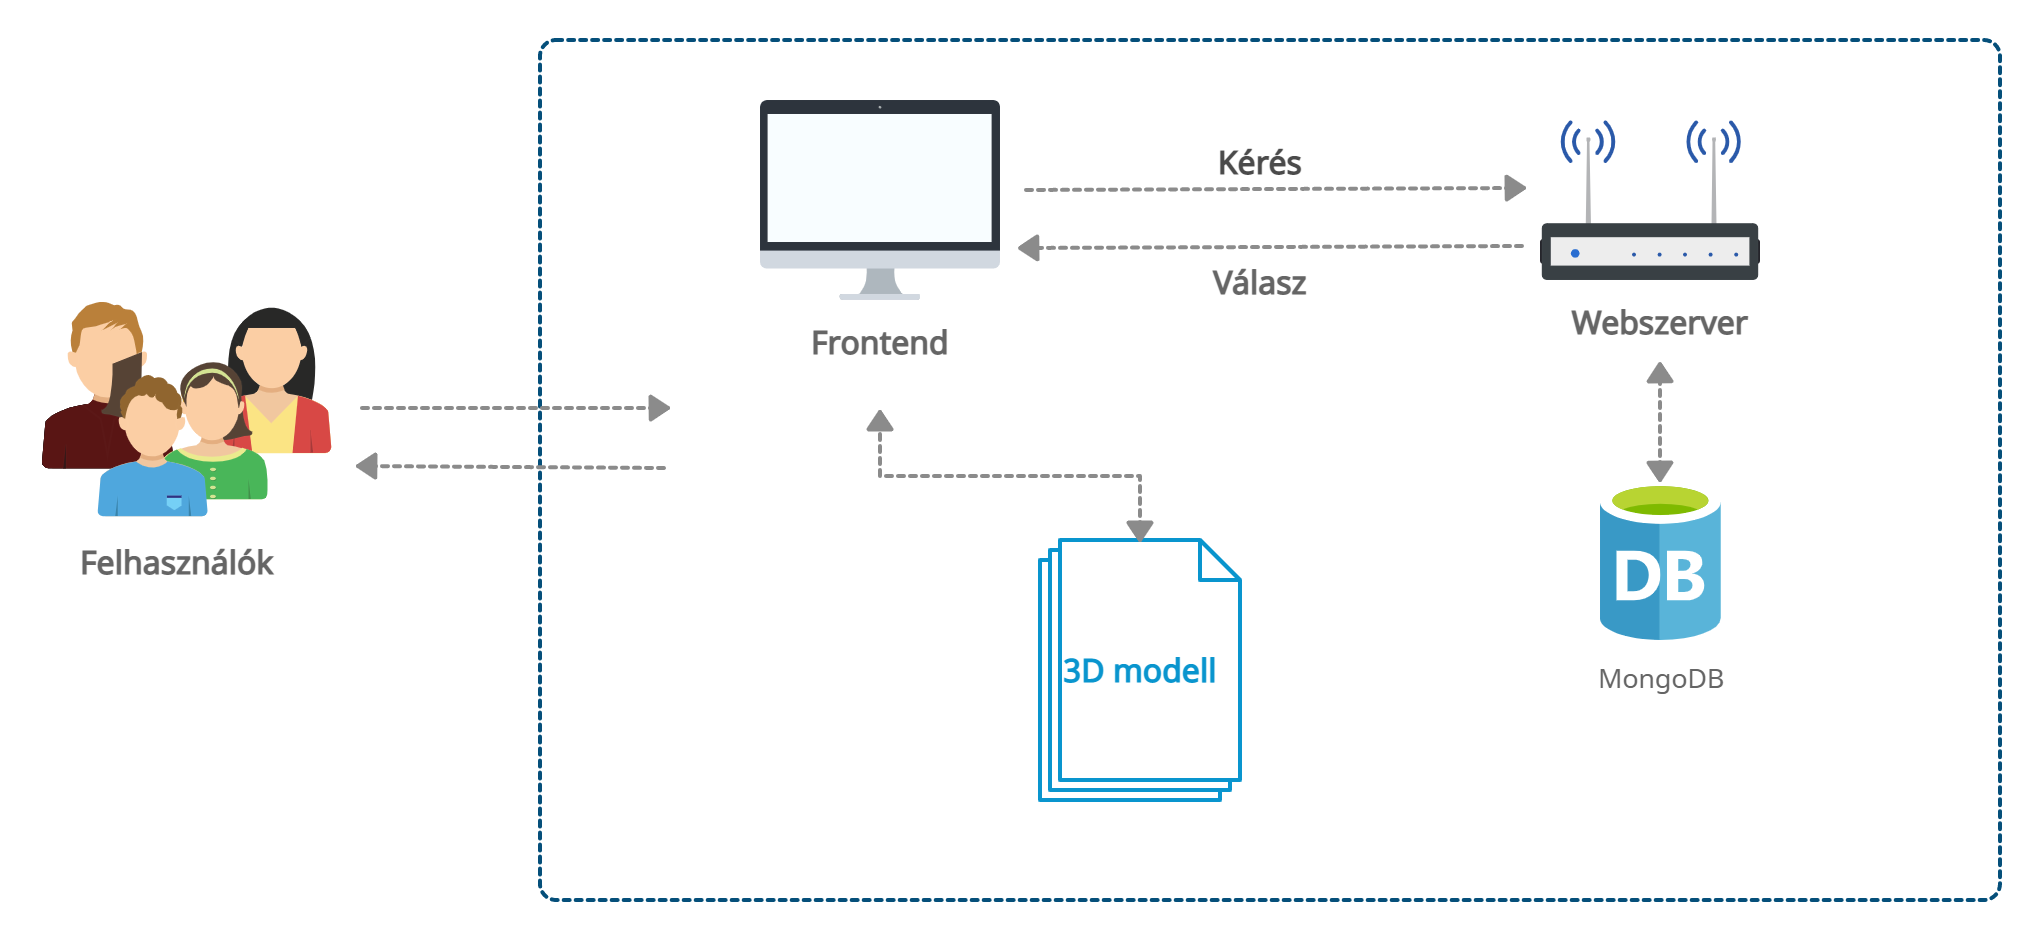
\includegraphics[width=1\linewidth]{figures/images/webalkalmazasarchitect.png}
	\caption[A webalkalmazás rendszer architektúrája]{\textit{A webalkalmazás rendszer architektúrája}}
	\label{fig:systemArchLittle}
\end{figure}